\chapter{Denní program přechodu}
\label{Program_prechodu}
%% -------------------------------------------------- %%
\def\figurename{Obr.} % Figure name
\def\tablename{Tab.} % Table name
\def\figureautorefname{obr.} % Autoreference 
\def\tableautorefname{tab.} % Autoreference
\def\chapterautorefname{kapitola} % Autoreference
%% -------------------------------------------------- %%

Celková délka horského treku činí 170\:km a je rozdělena do několika etap, které vedou přes 7 údolí. Existuje hned několik variant, ze kterých si můžeme vybrat.
Moje doporučení je varianta s 11 etapami. Každá etapa má průměrnou délku přibližně 13-20\:km a trvá kolem 7-9 hodin denně. Většina turistů absolvuje jednu etapu za den, zatímco zkušenější turisti ji zvládnou i rychleji. Nicméně někteří mohou zvolit jinou trasu, postupující v klidnějším tempu, která může trvat až 14 dní. Většina lidí volí navigovat stezku proti směru hodinových ručiček, aby si mohli užít co nejvíce výhledů na Mont Blanc. 

V následujících podkapitolách uvádím podrobnosti o každé etapě. V káždé etapě je popsán denní program přechodu a to konkrétněji výchozí a koncový bod, denní převýšení, délka denních etap, časové plánování. Údaje o místech k přespání (horské chaty, bivaky), dostupnost vody, elektřiny, mobilního signálu, nouzová sestupová místa a případném doplňování zásob. Také je možnost si vybrat variantu s přespáním ve stanu. V tom případě by bylo možno trasu upravovat dle fyzické kondici.
\section{Etapa 1}
\subsubsection*{Celková délka}
\noindent Vzdálenost: 15,5\:km
\subsubsection*{Výchozí a koncový bod}
\noindent Výchozí bod: Les Houches
\noindent Koncový bod: Les Contamines
\subsubsection*{Převýšení}
\noindent Vystoupáno: 1\:489\:m
\noindent Sestoupáno: 788\:m
\subsubsection*{Časové plánování}
\noindent Předpokládaný čas túry: 7-9 hod.

První etapa bude na začátek náročnější. Bude nás čekat téměř 16,0\:km s vystoupáním 1\:489\:m a s klesáním 788\:m. Předpokládaný čas této etapy bude záviset na fyzické kondici účastněných. Předpokládám rozpětí mezi 7-9 hodinami.
\subsubsection*{Cena ubytování}
\noindent Uvedená cena je podle ceníku pro rok 2024
\noindent Cena: 43,0\:€ 
\noindent Prázdninová taxa: 0,80\:€

V ceně je zahrnuto ubytování a polopenze (večeře a snídaně)
\subsubsection*{Nouzová sestupová místa}
Pokud by byl nějaký problém v první etapě, nouzový sestup bych volila stejnou cestou zpět k autu.
\subsubsection*{Další informace}
Po 7,1\:km nás bude čekat vyhlídkové místo. Za dalších 4,8\:km se dostaneme do sedla Col de Tricot (2\:120\:m) a odtud bude zbývat 3,6\:km do cíle této etapy.
%% -------------------------------------------------- %%
%% -------------------- Picture --------------------- %%
%% -------------------------------------------------- %%
\begin{figure}[!hbt]
    \centering
    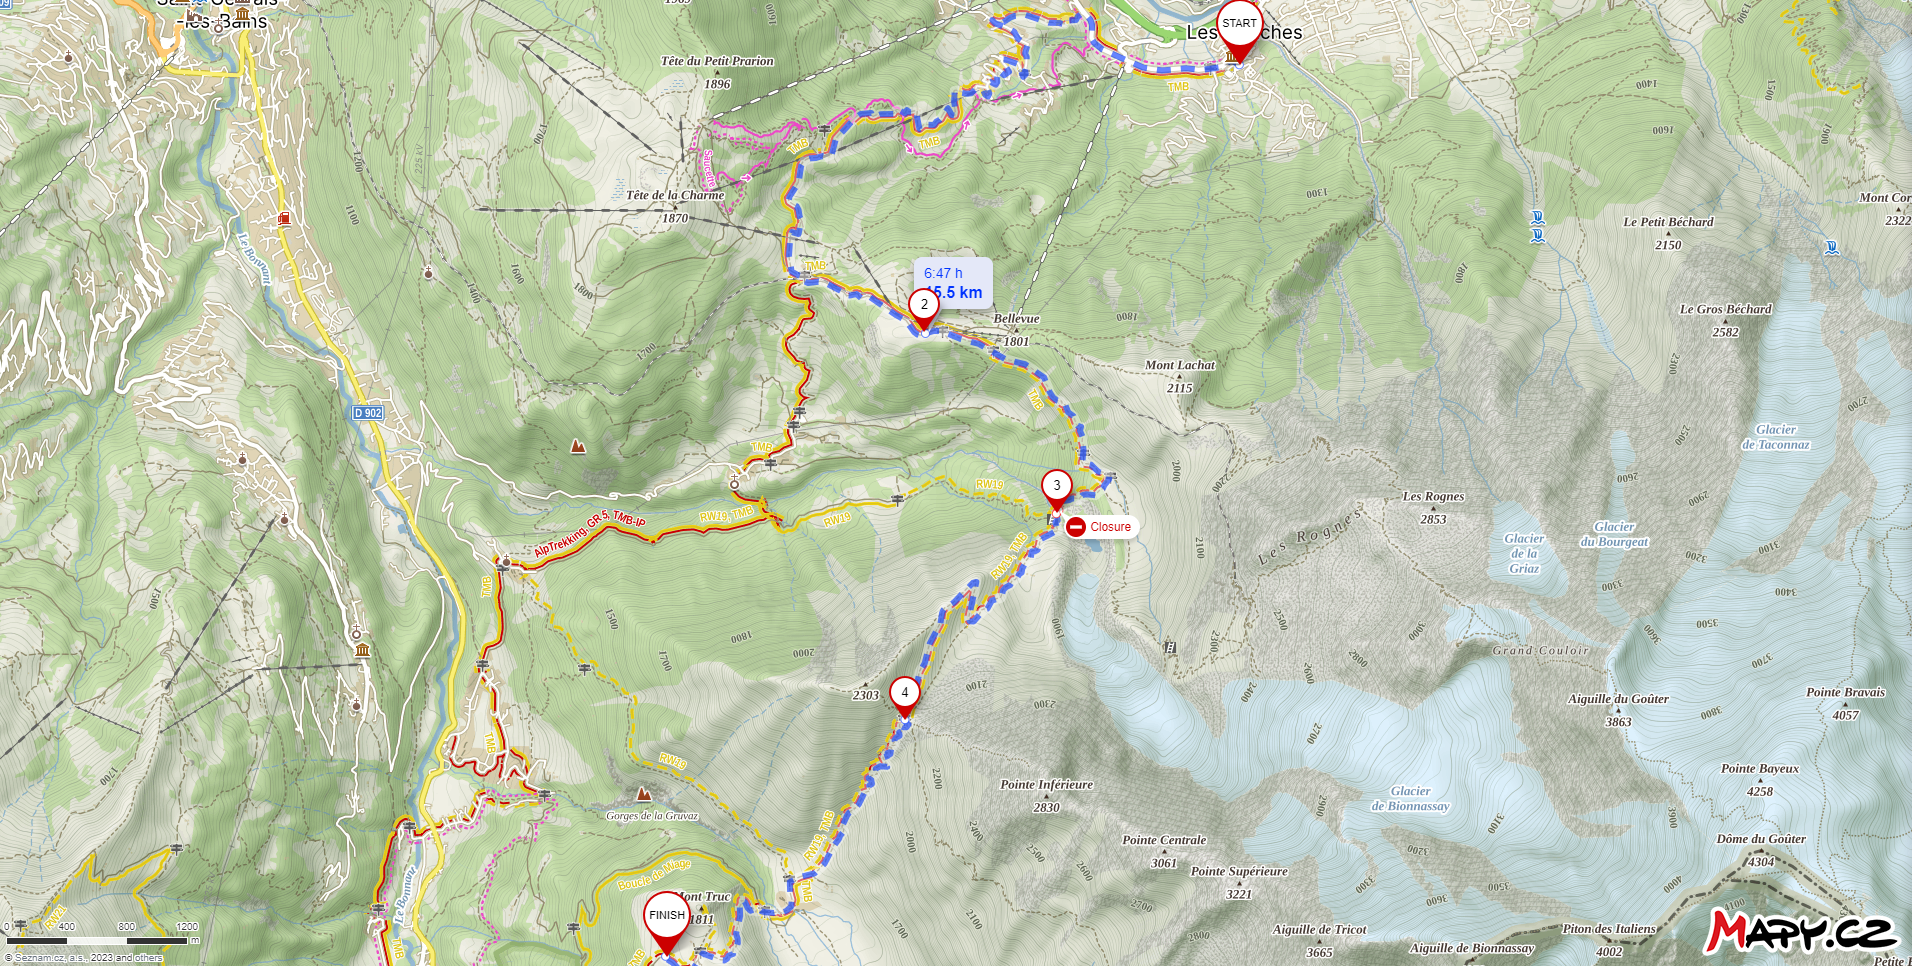
\includegraphics[width=10.0cm]{Figures/day_1.png}
    \caption[Trasa: den první]{Trasa 1. etapy (mapa převzata ze zdroje mapy.cz)}
    \label{Obr:day_1}
\end{figure} 
%% -------------------------------------------------- %%
\section{Etapa 2}
\subsubsection*{Celková délka}
\noindent Vzdálenost:22,6\:km
\subsubsection*{Výchozí a koncový bod}
\noindent Výchozí bod: Les Contamines
\noindent Koncový bod: Les Chapieux
\subsubsection*{Převýšení}
\noindent Vystoupáno: 1\:337\:m
\noindent Sestoupáno: 1\:476\:m
\subsubsection*{Časové plánování}
\noindent Předpokládaný čas túry: 9-11 hod.

Pokračujeme druhou náročnější etapou, která bude mít téměř 23,0\:km s vystoupáním 1337\:m výškových a sestoupáno budeme mít 1476\:m. Tuto etapu odhaduji na 9-11 hodin. Tato etapa bude náročnější než první, a proto očekávám pomalejší tempo.
\subsubsection*{Cena ubytování}
\noindent Uvedená cena je podle ceníku pro rok 2024
\noindent Cena:
\begin{itemize}
	\item Pokoj s polopenzí (sprcha a WC) 84,12\:€
	\item Pokoj s polopenzí (sprcha a WC nahoře) 79,12\:€
	\item Noclehárna s polopenzí 65,12\:€
	\item Prázdninová taxa 0,88\:€
\end{itemize}

\noindent Kemp: zdarma

\subsubsection*{Nouzová sestupová místa}
Druhá etapa prochází Les Contamines a dále etapa končí nedaleko silnice. Pokud by byl nějaký problém v této etapě, volila bych stejnou cestou se dostat k nejbližšímu bodu a to buď Les Contamines a nebo k silnici a odtud dále zpět k autu.
\subsubsection*{Další informace}
Po 11,3\:km nás bude čekat chata Refuge de la Balme, ve které bude možnost se občerstvit, popřípadě si odpočinout. Po 2,3\:km nás bude čekat pramen vody, kde bude možnost dočerpat vodu, popřípadě se napít. Po 1,4\:km nás čeká sedlo Abri du Col de Bonhomme (2\:329\:m), kde bude také turistický přístřešek, kde budeme moct posedět a nabrat další síly. Po 2,0\:km nás bude opět čekat chata Refuge du col de la Croix du Bonhomme a vrchol Col de la croix du bonhomme (2\:433\:m) a poté už bude zbývat pouhých 5,5\:km do cíle této etapy.
%% -------------------------------------------------- %%
%% -------------------- Picture --------------------- %%
%% -------------------------------------------------- %%
\begin{figure}[!hbt]
    \centering
    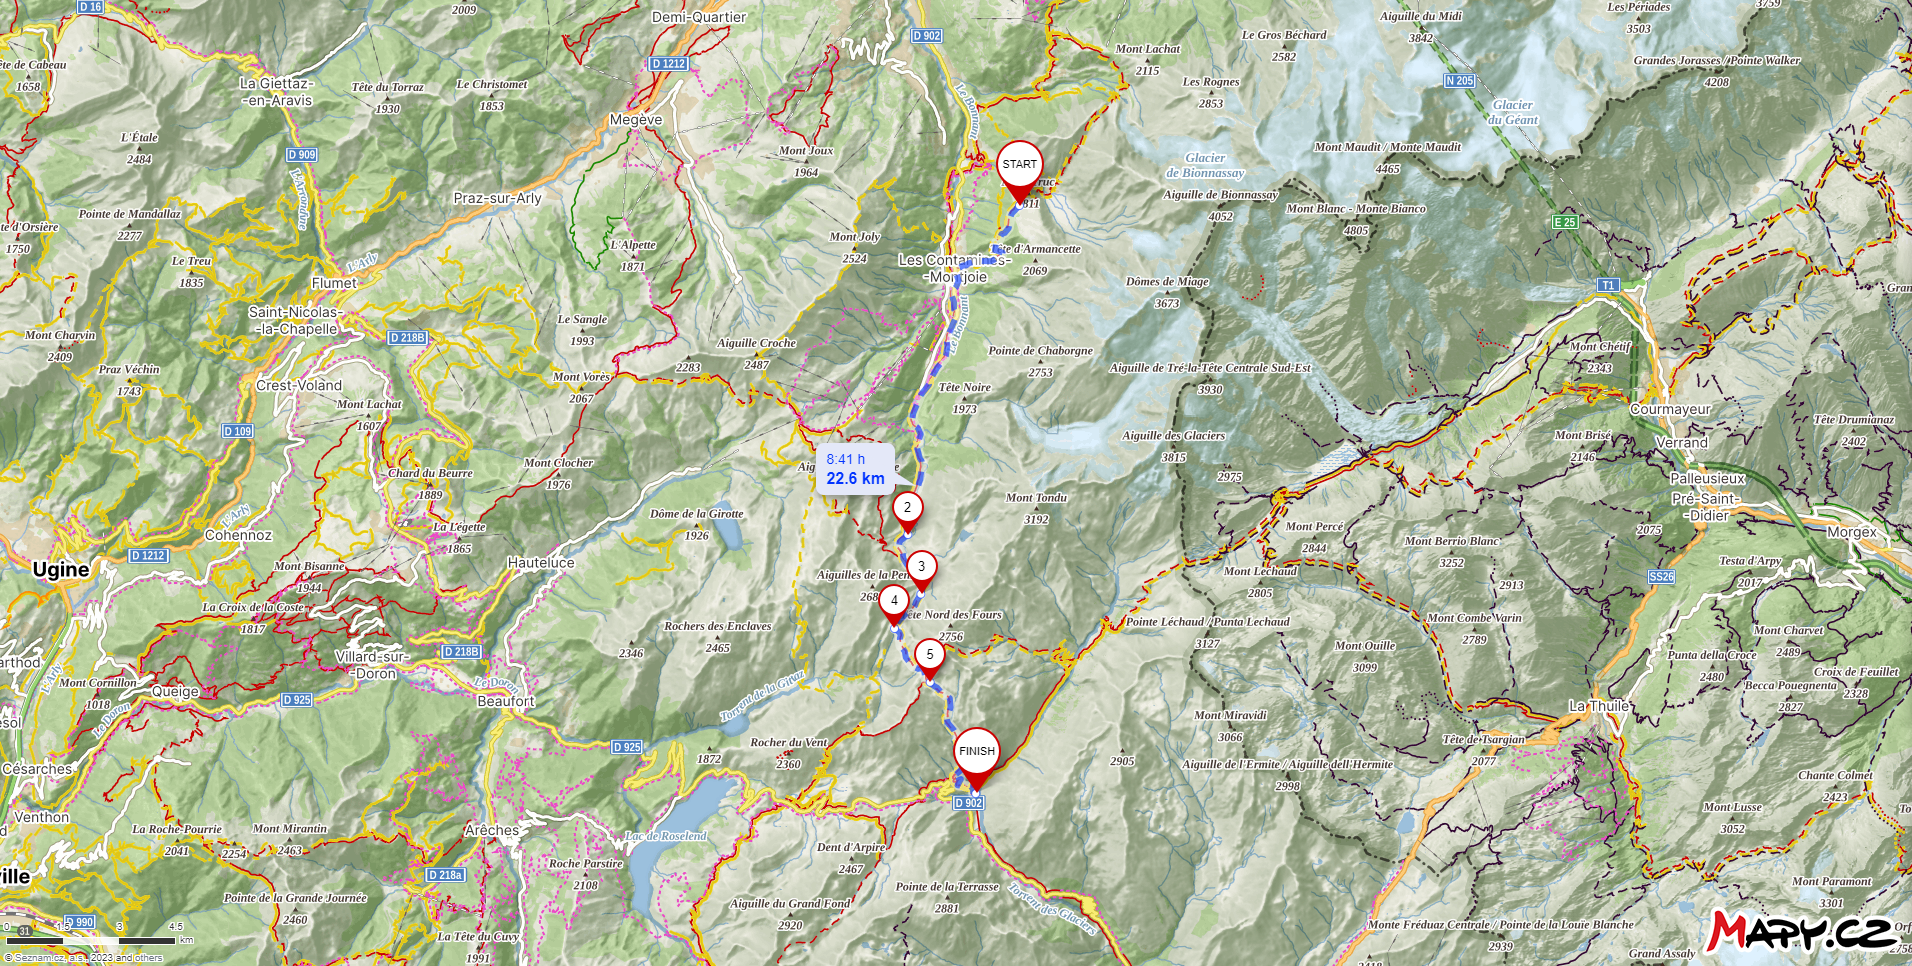
\includegraphics[width=10.0cm]{Figures/day_2.png}
    \caption[Trasa: den druhý]{Trasa 2. etapy (mapa převzata ze zdroje mapy.cz)}
    \label{Obr:day_2}
\end{figure} 
%% -------------------------------------------------- %%
\section{Etapa 3}
\subsubsection*{Celková délka}
\noindent Vzdálenost: 14,2\:km
\subsubsection*{Výchozí a koncový bod}
\noindent Výchozí bod: Les Chapieux
\noindent Koncový bod: Rifugio Elisabetta
\subsubsection*{Převýšení}
\noindent Vystoupáno: 1\:026\:m
\noindent Sestoupáno: 379\:m
\subsubsection*{Časové plánování}
\noindent Předpokládaný čas túry: 6-8 hod.

V této etapě nás čeká 14,0\:km, bude to znatelně jednodušší od předchozích prvních dvou náročných etapách. Stále, ale vystoupáme 1\:026\:m a sestoupáme 379\:m.
\subsubsection*{Cena ubytování}
\noindent Uvedená cena je podle ceníku pro rok 2023
\noindent Cena:
\begin{itemize}
	\item Noclehárna s polopenzí členové 46\:€ a nečlenové 54\:€
	\item Pokoj s polopenzí (4-7 osob) členové 52\:€ a nečlenové 60\:€
	\item Polopenze Dvoulůžkový pokoj členové 60\:€ a nečlenové 68\:€
\end{itemize}
\subsubsection*{Nouzová sestupová místa}
Třetí etapa nenabízí jiné varianty sestupu, a proto i tady bych volila cestu zpět.
\subsubsection*{Další informace}
V této etapě budeme přecházet hranice Francie a Itálie po cca 10,7\:km od startu. Další etapa nás tedy provede Itálií. 
%% -------------------------------------------------- %%
%% -------------------- Picture --------------------- %%
%% -------------------------------------------------- %%
\begin{figure}[!hbt]
    \centering
    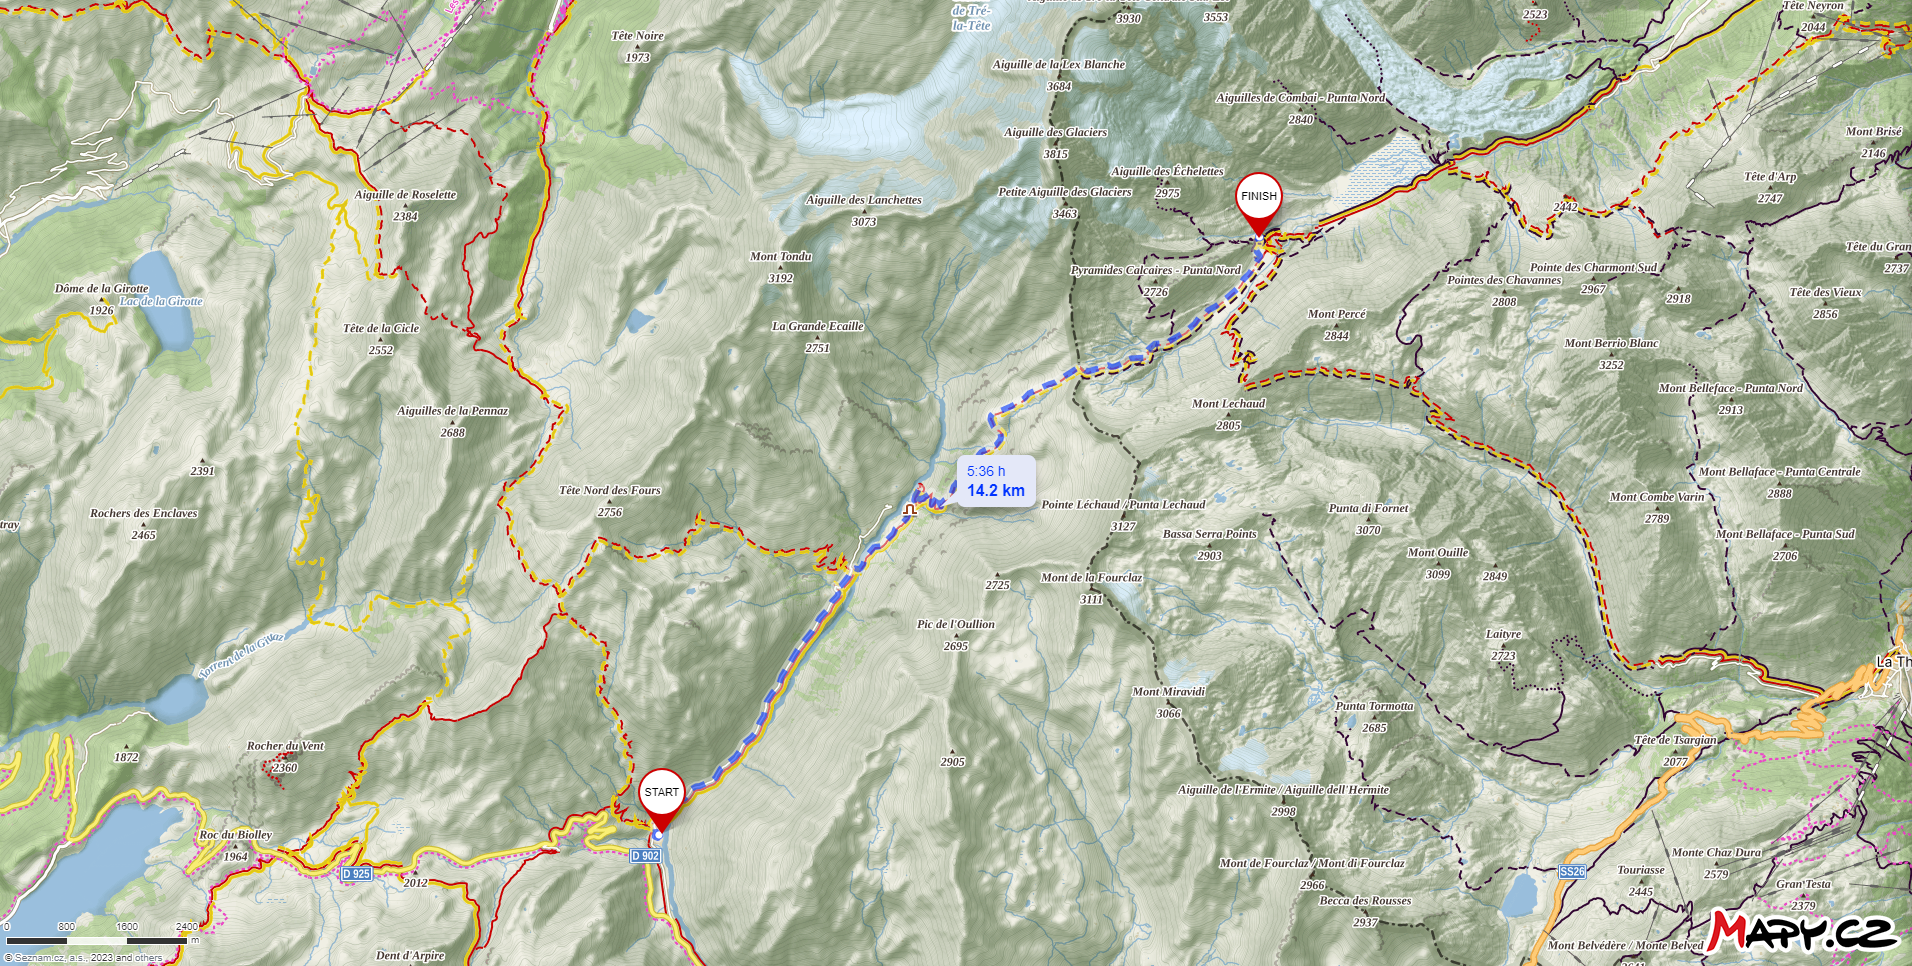
\includegraphics[width=10.0cm]{Figures/day_3.png}
    \caption[Trasa: den třetí]{Trasa 3. etapy (mapa převzata ze zdroje mapy.cz)}
    \label{Obr:day_3}
\end{figure} 
%% -------------------------------------------------- %%
\section{Etapa 4}
\subsubsection*{Celková délka}
\noindent Vzdálenost: 19,3\:km
\subsubsection*{Výchozí a koncový bod}
\noindent Výchozí bod: Refugio Elisabetta 
\noindent Koncový bod: Courmayeur
\subsubsection*{Převýšení}
\noindent Vystoupáno: 1\:290\:m
\noindent Sestoupáno: 1\:512\:m
\subsubsection*{Časové plánování}
\noindent Předpokládaný čas túry: 8-10 hod.

Etapa 4 opět nebude jednoduchá. Vzdálenost túry bude 19,3\:km s vystoupáním 1290\:m a sestoupáme 1512\:m.
\subsubsection*{Cena ubytování}
\noindent Cena:
\begin{itemize}
	\item Prázdninová taxa 1,00\:€
	\item Polopenze na koleji 16 px 65,00\:€ na osobu včetně večeře, noclehu, snídaně a sprchy na znamení
	\item Polopenze na koleji 12 px 65,00\:€ na osobu včetně večeře, noclehu, snídaně a sprchy na znamení
	\item Pokoj s polopenzí 80,00\:€ na osobu včetně večeře, lůžka, snídaně a sprchy na znamení
	\item Polopenze Pokoj s povlečením 95,00\:€ na osobu včetně večeře, lůžka, snídaně a sprchy
\end{itemize}
\subsubsection*{Nouzová sestupová místa}
Zde je možnost jít jinou cestou a to spodní se vzdáleností 18,9\:km a s vystoupáním 836\:m a se sestoupáním 1059\:m. Rozdíl ve vzdálenosti by byl pouhých 400\:m. Vystoupaných metrů bychom měli o 454\:m a sestoupaných bychom měli o 453\:m méně.
\subsubsection*{Další informace}
V této etapě potkáme dvě chaty, které od sebe budou 700\:m. První nás čeká po 10,2\:km Rifugio - Restaurante Maison Vieille.
%% -------------------------------------------------- %%
%% -------------------- Picture --------------------- %%
%% -------------------------------------------------- %%
\begin{figure}[!hbt]
    \centering
    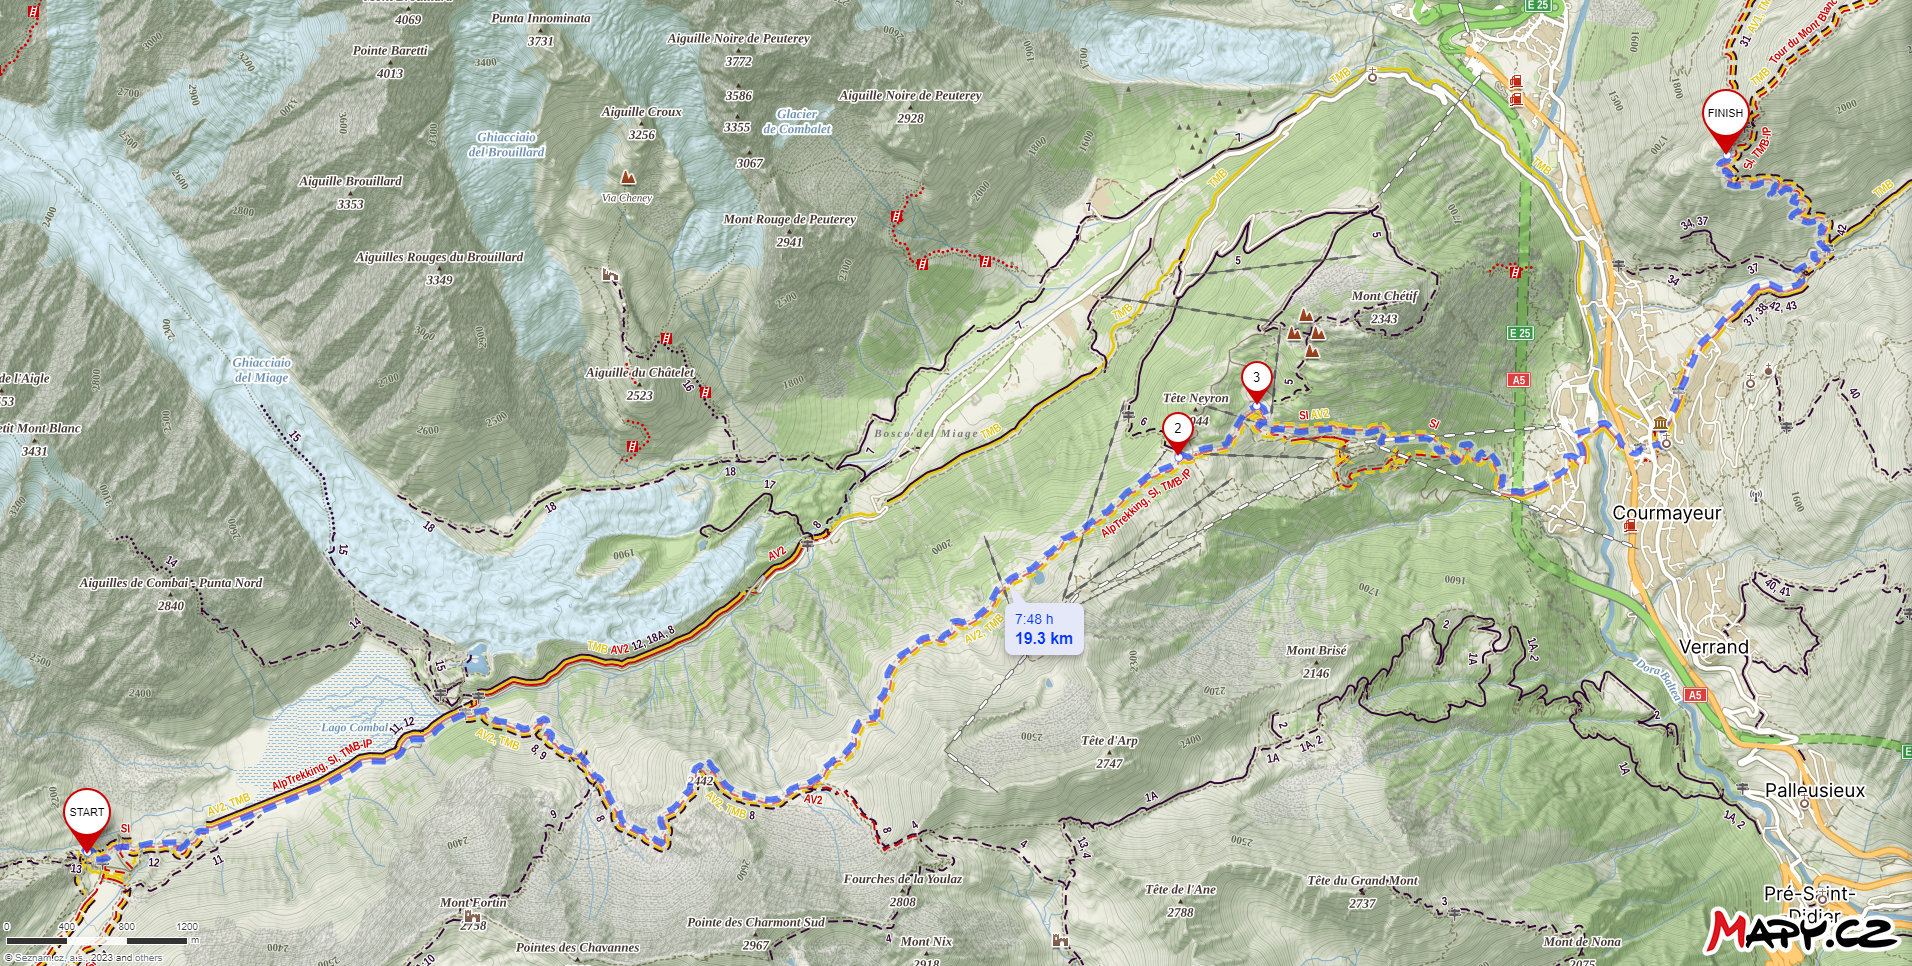
\includegraphics[width=10.0cm]{Figures/day_4.png}
    \caption[Trasa: den čtvrtý]{Trasa 4. etapy (mapa převzata ze zdroje mapy.cz)}
    \label{Obr:day_4}
\end{figure} 
%% -------------------------------------------------- %%
\section{Etapa 5}
\subsubsection*{Celková délka}
\noindent Vzdálenost: 10,5 km
\subsubsection*{Výchozí a koncový bod}
\noindent Výchozí bod: Courmayeur
\noindent Koncový bod: Rifugio Bonatti
\subsubsection*{Převýšení}
\noindent Vystoupáno: 885 m
\noindent Sestoupáno: 827 m
\subsubsection*{Časové plánování}
\noindent Předpokládaný čas túry: 5-7 hod.

Etapa 5 bude zase spíše odpočinková. Čeká nás 10,5\:km a vystoupáme 885\:m a sestoupáme 827\:m.
\subsubsection*{Cena ubytování}
\noindent Uvedená cena je podle ceníku pro rok 2023
\noindent Cena:
\begin{itemize}
	\item Lůžko ve 2 - 4 lůžkovém pokoji 40,00\:€
	\item Lůžko v pokoji s více než 4 lůžky 40,00\:€
	\item Polopenze (cena za osobu) 65,00\:€
	
\end{itemize}
\subsubsection*{Nouzová sestupová místa}
Pátá etapa nabízí kratší variantu, která by byla dlouhá 7,6\:km a vystoupalo by se pohých 335\:m a sestoupalo by se 279\:m. Tato varianta by tedy byla kratší o 2,9\:km, vystoupáno by bylo o 550\:m méně a sestoupáno by bylo o 548\:m méně. Pokud by byl nějaký problém bylo by možné se vrátit do Courmayeur.
\subsubsection*{Další informace}
Po 4,8\:km nás bude čekat sedlo Col Sapin (2\:435\:m) a po dalších 2,4\:km sedlo Refuge Walter-Bonatti (2\:524\:m).
%% -------------------------------------------------- %%
%% -------------------- Picture --------------------- %%
%% -------------------------------------------------- %%
\begin{figure}[!hbt]
    \centering
    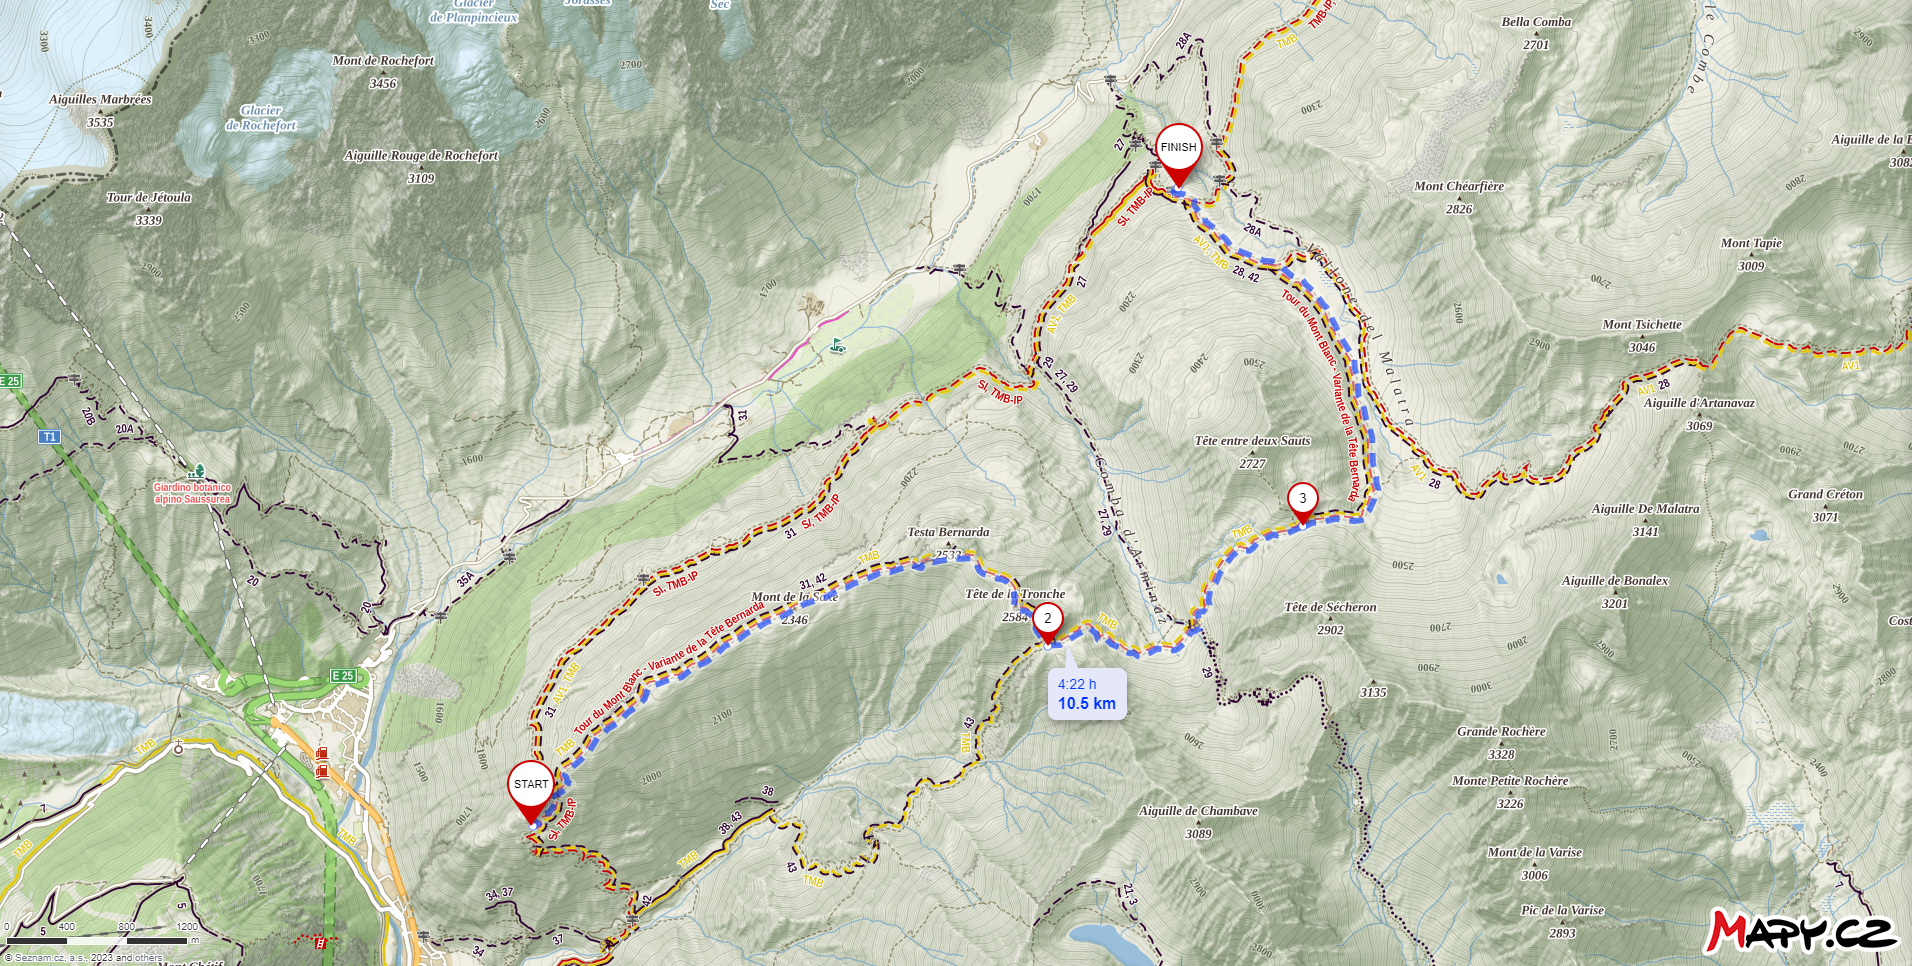
\includegraphics[width=10.0cm]{Figures/day_5.png}
    \caption[Trasa: den pátý]{Trasa 5. etapy (mapa převzata ze zdroje mapy.cz)}
    \label{Obr:day_5}
\end{figure} 
%% -------------------------------------------------- %%
\section{Etapa 6}
\subsubsection*{Celková délka}
\noindent Vzdálenost: 19,5\:km
\subsubsection*{Výchozí a koncový bod}
\noindent Výchozí bod: Rifugio Bonatti 
\noindent Koncový bod: La Fouly
\subsubsection*{Převýšení}
\noindent Vystoupáno: 908\:m
\noindent Sestoupáno: 1\:340\:m
\subsubsection*{Časové plánování}
\noindent Předpokládaný čas túry: 8-10 hod.

Etapa 6 bude vzdáleností 19,5\:km řazena mezi delší, ale nastoupáme pouze 908\:m a sestoupáme 1340\:m.
\subsubsection*{Cena ubytování}
\noindent Uvedená cena je podle ceníku pro rok 2023
\noindent Cena:
\begin{itemize}
	\item Prázdninová taxa 1,6\:€
	\item Využití místního stanu 30\:€
	\item Dospělí 9\:€ (v sezóně červenec-srpen) a 7,2\:€ (mimo sezónu květen, červen, září)
	\item umístění vlastního stanu 16\:€
\end{itemize}
\subsubsection*{Nouzová sestupová místa}
V šesté etapě se dostaneme do La Fouly, takže pokud bude nějaký problém bude nejlepší dojít. Zde žádné jiné varianty cesty nejsou.
\subsubsection*{Další informace}
Po 7,7\:km dojdeme k chatě Refuge Elena, zde bude možno se občerstvit a odpočinout. Dále po 2,3\:km přejdeme hranice s Itálií a Švýcarskem a od té doby nás bude čekat trasa vedena Švýcarskem. Po 3,6\:km bude opět možnost zastavit na chatě La Peule. Poté už nám bude zbývat pohých 5,9\:km.
%% -------------------------------------------------- %%
%% -------------------- Picture --------------------- %%
%% -------------------------------------------------- %%
\begin{figure}[!hbt]
    \centering
    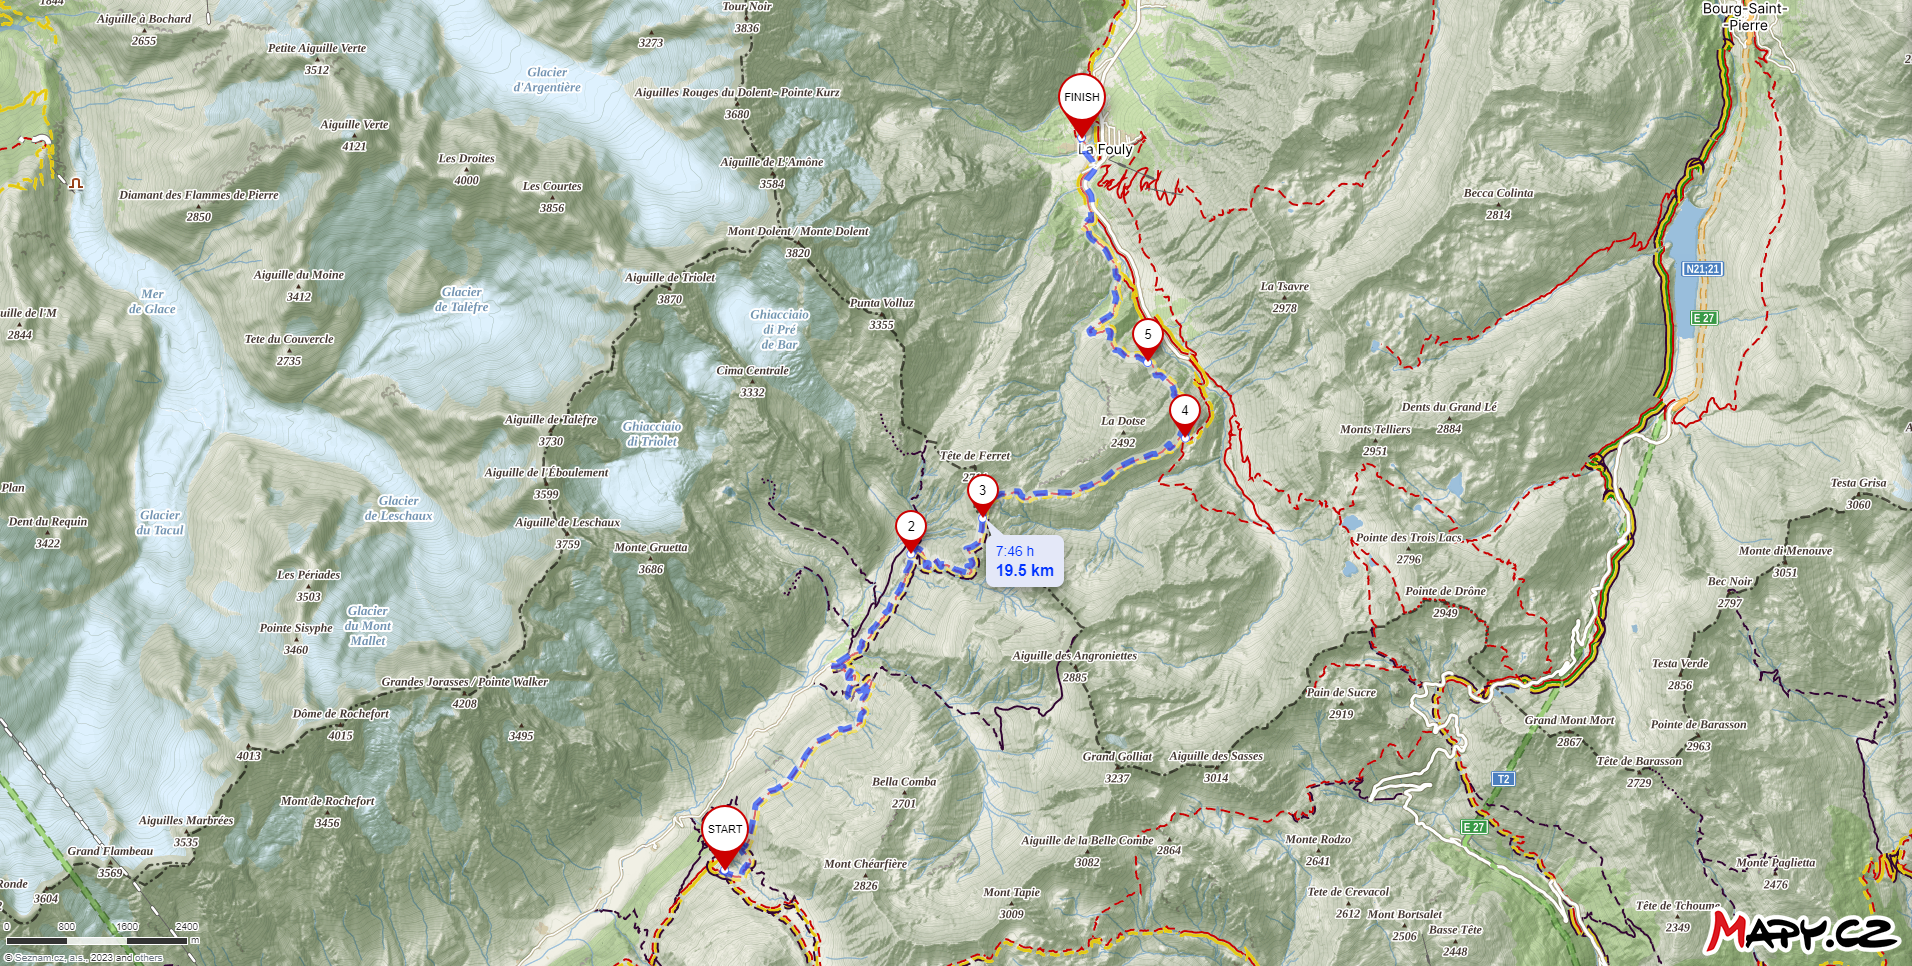
\includegraphics[width=10.0cm]{Figures/day_6.png}
    \caption[Trasa: den šestý]{Trasa 6. etapy (mapa převzata ze zdroje mapy.cz)}
    \label{Obr:day_6}
\end{figure} 
%% -------------------------------------------------- %%
\section{Etapa 7}
\subsubsection*{Celková délka}
\noindent Vzdálenost: 15,2\:km
\subsubsection*{Výchozí a koncový bod}
\noindent Výchozí bod: La Fouly
\noindent Koncový bod: Champex-Lac
\subsubsection*{Převýšení}
\noindent Vystoupáno: 474\:m
\noindent Sestoupáno: 584\:m
\subsubsection*{Časové plánování}
\noindent Předpokládaný čas túry: 6-8 hod.

Etapa 7 nebude nijak extra náročná, čeká nás 15,2\:km s vystoupáním 474\:m a sestoupáním 584\:m.
\subsubsection*{Cena ubytování}
\noindent Uvedená cena je podle ceníku pro rok 2023
\noindent Cena v kempu s vlastním stanem
\noindent Cena:
\begin{itemize}
	\item Prázdninová taxa 1,6\:CHF
	\item Dospělí 9\:CHF
	\item Stan 16\:CHF
\end{itemize}

\noindent Uvedená cena je podle ceníku pro rok 2024
\noindent Cena:
\begin{itemize}
	\item Pagoda (stan s lůžkem + nafukovací matrace + deka) = 24\:CHF + daň (61\:CHF + daň v polopenzi)
	\item Velká noclehárna (18 lůžek) = 34\:CHF + daň (71\:CHF + daň s polopenzí)
	\item Malá noclehárna (6 lůžek) = 44 CHF + daň (81 CHF + daň s polopenzí)
	\item Dvoulůžkový pokoj s vlastní venkovní sprchou a WC = 53\:CHF / osoba + daň (90\:CHF / osoba + daň v polopenzi)
	\item 3lůžkový pokoj s vlastní sprchou a WC venku = 53\:CHF / osoba + daň (90\:CHF / osoba + daň v polopenzi)
	\item Dvoulůžkový pokoj, sprcha a vnitřní WC = 58\:CHF / osoba + daň (95\:CHF / osoba + daň v polopenzi)
\end{itemize}
\subsubsection*{Nouzová sestupová místa}
Tato varianta vede podel silnice a prochází několika vesnicemi a končí v Champex-Lax. Pokud by na cestě nastal problém, dostala bych se nejkratší cestou na silnici a odtud pokračovala dopravou.
\subsubsection*{Další informace}
Po 12,4\:km bude pramen vody, ze kterého se budeme moct napít popřípadě doplnit vodu.
%% -------------------------------------------------- %%
%% -------------------- Picture --------------------- %%
%% -------------------------------------------------- %%
\begin{figure}[!hbt]
    \centering
    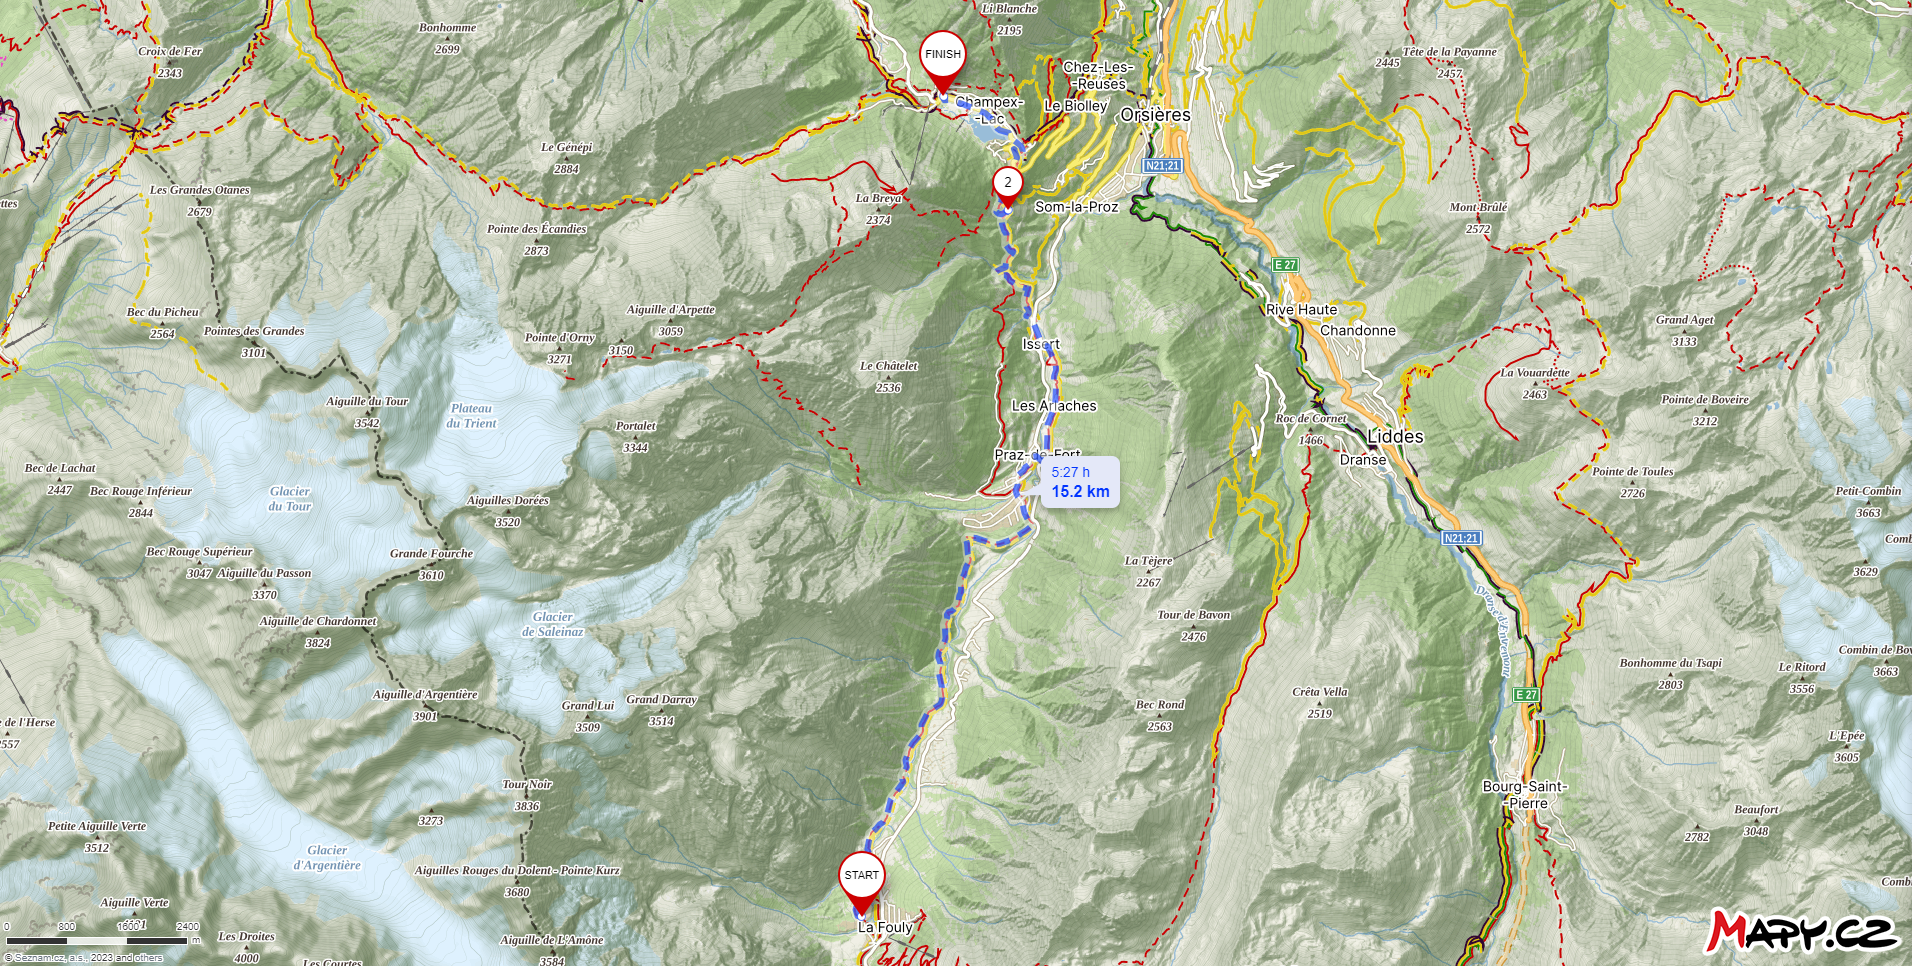
\includegraphics[width=10.0cm]{Figures/day_7.png}
    \caption[Trasa: den sedmý]{Trasa 7. etapy (mapa převzata ze zdroje mapy.cz)}
    \label{Obr:day_7}
\end{figure} 
%% -------------------------------------------------- %%
\section{Etapa 8}
\subsubsection*{Celková délka}
\noindent Vzdálenost: 16,3\:km
\subsubsection*{Výchozí a koncový bod}
\noindent Výchozí bod: Champex-Lac
\noindent Koncový bod: Trient
\subsubsection*{Převýšení}
\noindent Vystoupáno: 1\:934\:m
\noindent Sestoupáno: 1\:209\:m
\subsubsection*{Časové plánování}
\noindent Předpokládaný čas túry: 7-9 hod.

Etapa 8 bude mít značné převýšení od předchozích etap, vlastně se bude jednat o etapu s nejvyšším stoupáním a to 1\:934\:m a sestoupáme 1\:209\:m. Vzdálenost bude 16,3\:km.
\subsubsection*{Cena ubytování}
\noindent Uvedená cena je podle ceníku pro rok 2023
\noindent Cena: Ubytování s polopenzí 57\:€
\subsubsection*{Nouzová sestupová místa}
Tato varianta nabízí pouze delší variantu. Dochází se do Vallorcine, pokud by byl na cestě problém šla bych nejkratší cestou do jedné z vesnic.
\subsubsection*{Další informace}
Po 6,5\:km dojdeme do sedla Fenêtre d'Arpette (2\:665\:m) a po 1,6\:km nás bude čekat přístřešek, kde si budeme moct sednout, odpočinout a popřípadě si dát něco malého k snědku. Po dalších 4,4\:km bude pramen, ze kterého se bude možno napít nebo popřípadě doplnit vodu. Tato etapa bude končit na hranicích Švýcarska a Francie. Další den tedy budeme pokračovat už zase Francií.
%% -------------------------------------------------- %%
%% -------------------- Picture --------------------- %%
%% -------------------------------------------------- %%
\begin{figure}[!hbt]
    \centering
    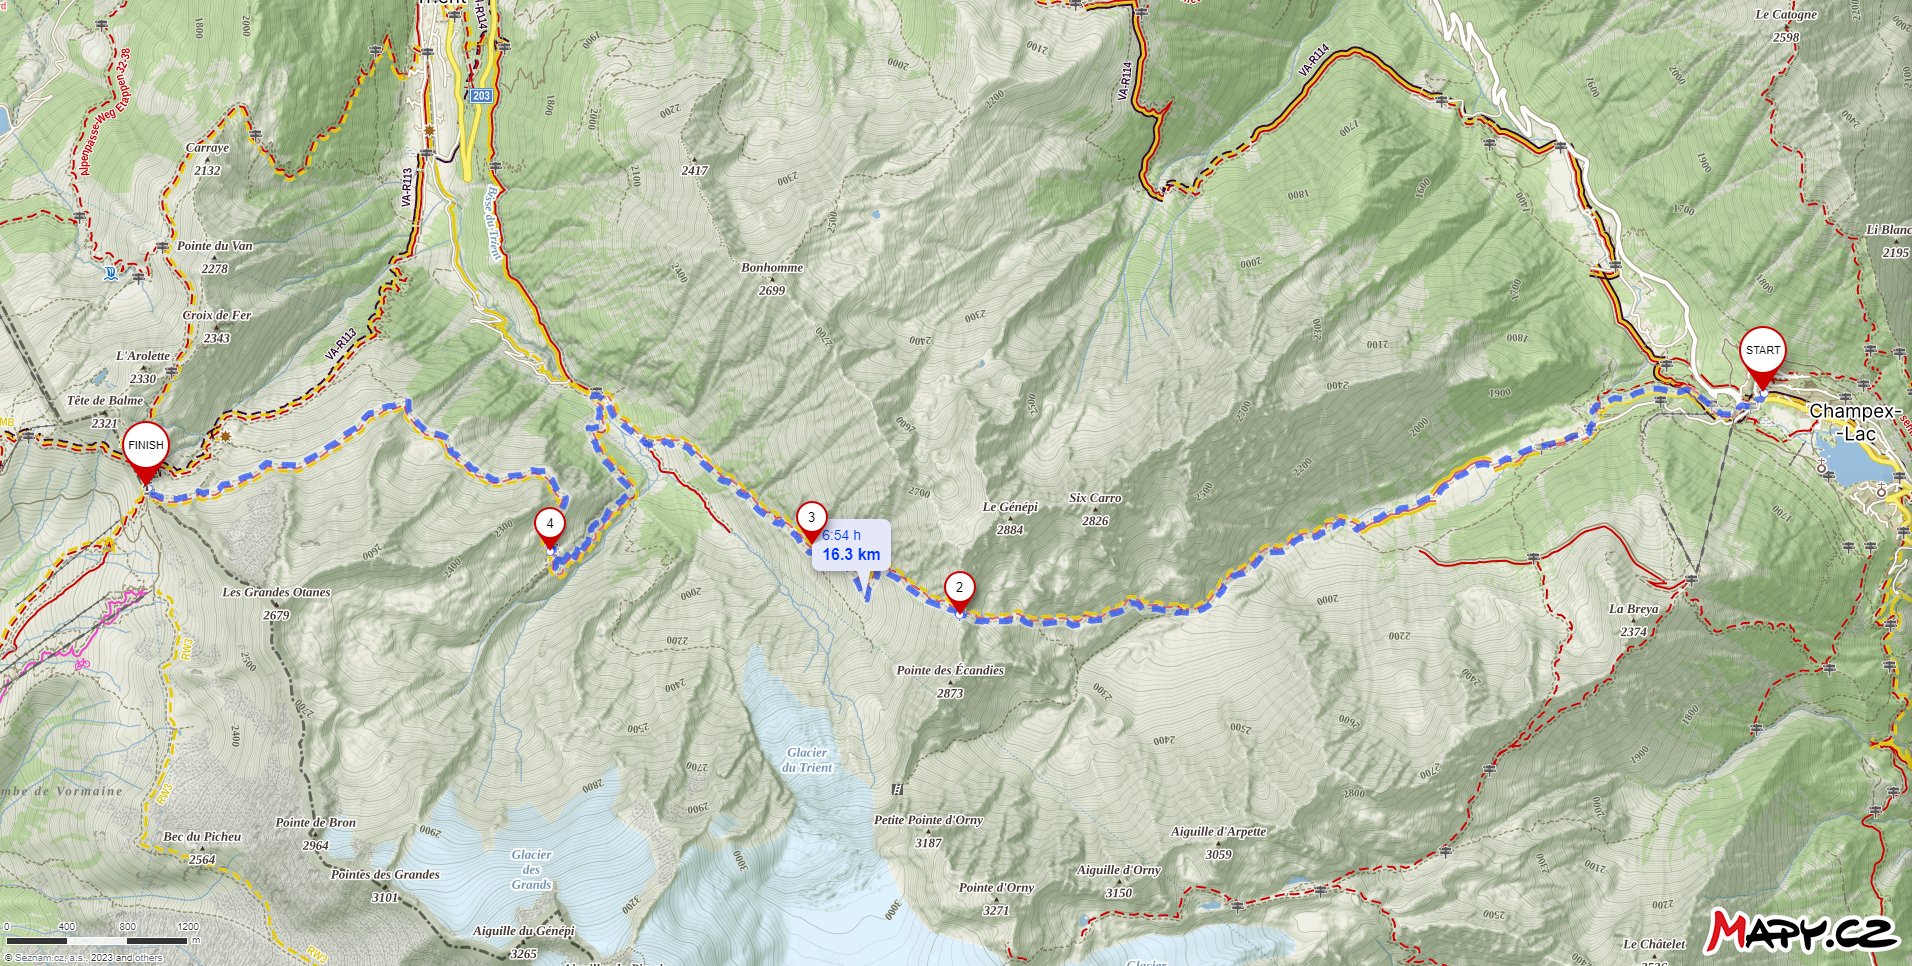
\includegraphics[width=10.0cm]{Figures/day_8.png}
    \caption[Trasa: den osmý]{Trasa 8. etapy (mapa převzata ze zdroje mapy.cz)}
    \label{Obr:day_8}
\end{figure} 
%% -------------------------------------------------- %%
\section{Etapa 9}
\subsubsection*{Celková délka}
\noindent Vzdálenost: 8,0\:km
\subsubsection*{Výchozí a koncový bod}
\noindent Výchozí bod: Trient
\noindent Koncový bod: Tré-le-Champ
\subsubsection*{Převýšení}
\noindent Vystoupáno: 190\:m
\noindent Sestoupáno: 997\:m
\subsubsection*{Časové plánování}
\noindent Předpokládaný čas túry: 3-5 hod.

Jelikož se nám celou dobu střídají náročnější etapy s odpočinkovějšími, tato nebude vyjímka. Po náročném předchozím stoupáním nás bude čekat pouhýchh 190\:m a sestoupáme 997\:m. Vzdálenost bude 8,0\:km. 
\subsubsection*{Cena ubytování}
\noindent Cena:
\begin{itemize}
	\item Ubytování s polopenzí 55\:€
	\item Stanování s polopenzí 40\:€
\end{itemize}
\subsubsection*{Nouzová sestupová místa}
Zde máme na výběr ze dvou cest, je možné absolvovat kratší, která má 6,0\:km, vystoupá se 26\:m a sestoupá se 838\:m. Cesta bude kratší o 2,0\:km, vystoupá se o 164\:m méně a sestoupá se o 159\:m méně. Cesta vede podel silnice na, které je několik autobusových zastávek.
\subsubsection*{Další informace}
Po 2,5\:km vystoupáme do sedla Col des Posettes (1\:997\:m). Po dalších 1,4\:km se dostaneme na vrchol Aiguillette des Posettes (2\:201\:m).
%% -------------------------------------------------- %%
%% -------------------- Picture --------------------- %%
%% -------------------------------------------------- %%
\begin{figure}[!hbt]
    \centering
    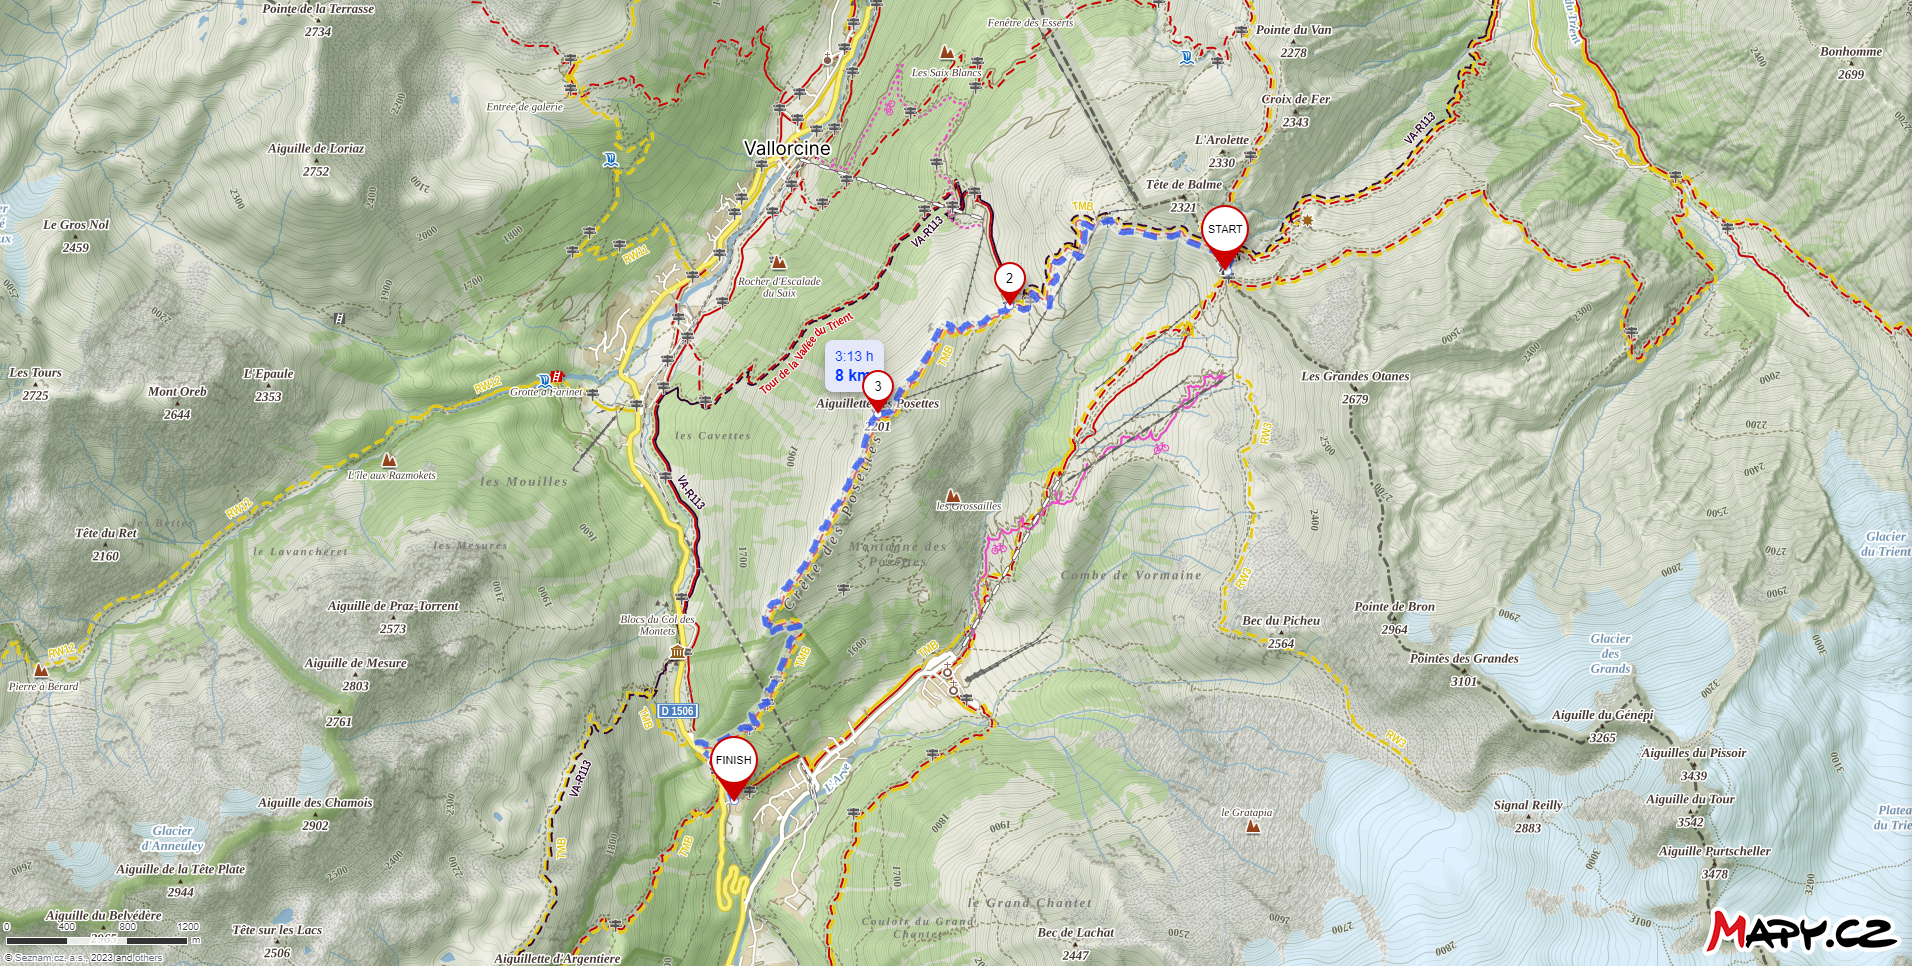
\includegraphics[width=10.0cm]{Figures/day_9.png}
    \caption[Trasa: den devátý]{Trasa 9. etapy (mapa převzata ze zdroje mapy.cz)}
    \label{Obr:day_9}
\end{figure} 
%% -------------------------------------------------- %%
\section{Etapa 10}
\subsubsection*{Celková délka}
\noindent Vzdálenost: 8,0\:km
\subsubsection*{Výchozí a koncový bod}
\noindent Výchozí bod: Tré-le-Champ 
\noindent Koncový bod: Flégère
\subsubsection*{Převýšení}
\noindent Vystoupáno: 960\:m
\noindent Sestoupáno: 463\:m
\subsubsection*{Časové plánování}
\noindent Předpokládaný čas túry: 4-6 hod.

Pomalu se budeme blížit k cíli. Čeká nás pouhých 8,0\:km s vystoupáním 960\:m a sestoupáním 463\:m.
\subsubsection*{Cena ubytování}
\noindent Uvedená cena je podle ceníku pro rok 2023
\noindent Cena: Ubytování s polopenzí 64\:€
\subsubsection*{Nouzová sestupová místa}
Opět zde máme variantu a to se vzdáleností 7,0\:km, vystoupáme 785\:km a sestoupáme 297\:km. Tato varianta bude o 1,0\:km kratší, vystoupá se 175\:m méně a sestoupá se o 166\:m méně.
\subsubsection*{Další informace}
Po 4,9\:km od startu nás budou čekat jezera Lac Blanc a chata Refuge du Lac Blanc, na které se budeme moct občerstvit. Budeme lehce za polovinou cesty a tak zde budeme moct setrvat delší dobu.
%% -------------------------------------------------- %%
%% -------------------- Picture --------------------- %%
%% -------------------------------------------------- %%
\begin{figure}[!hbt]
	\centering
	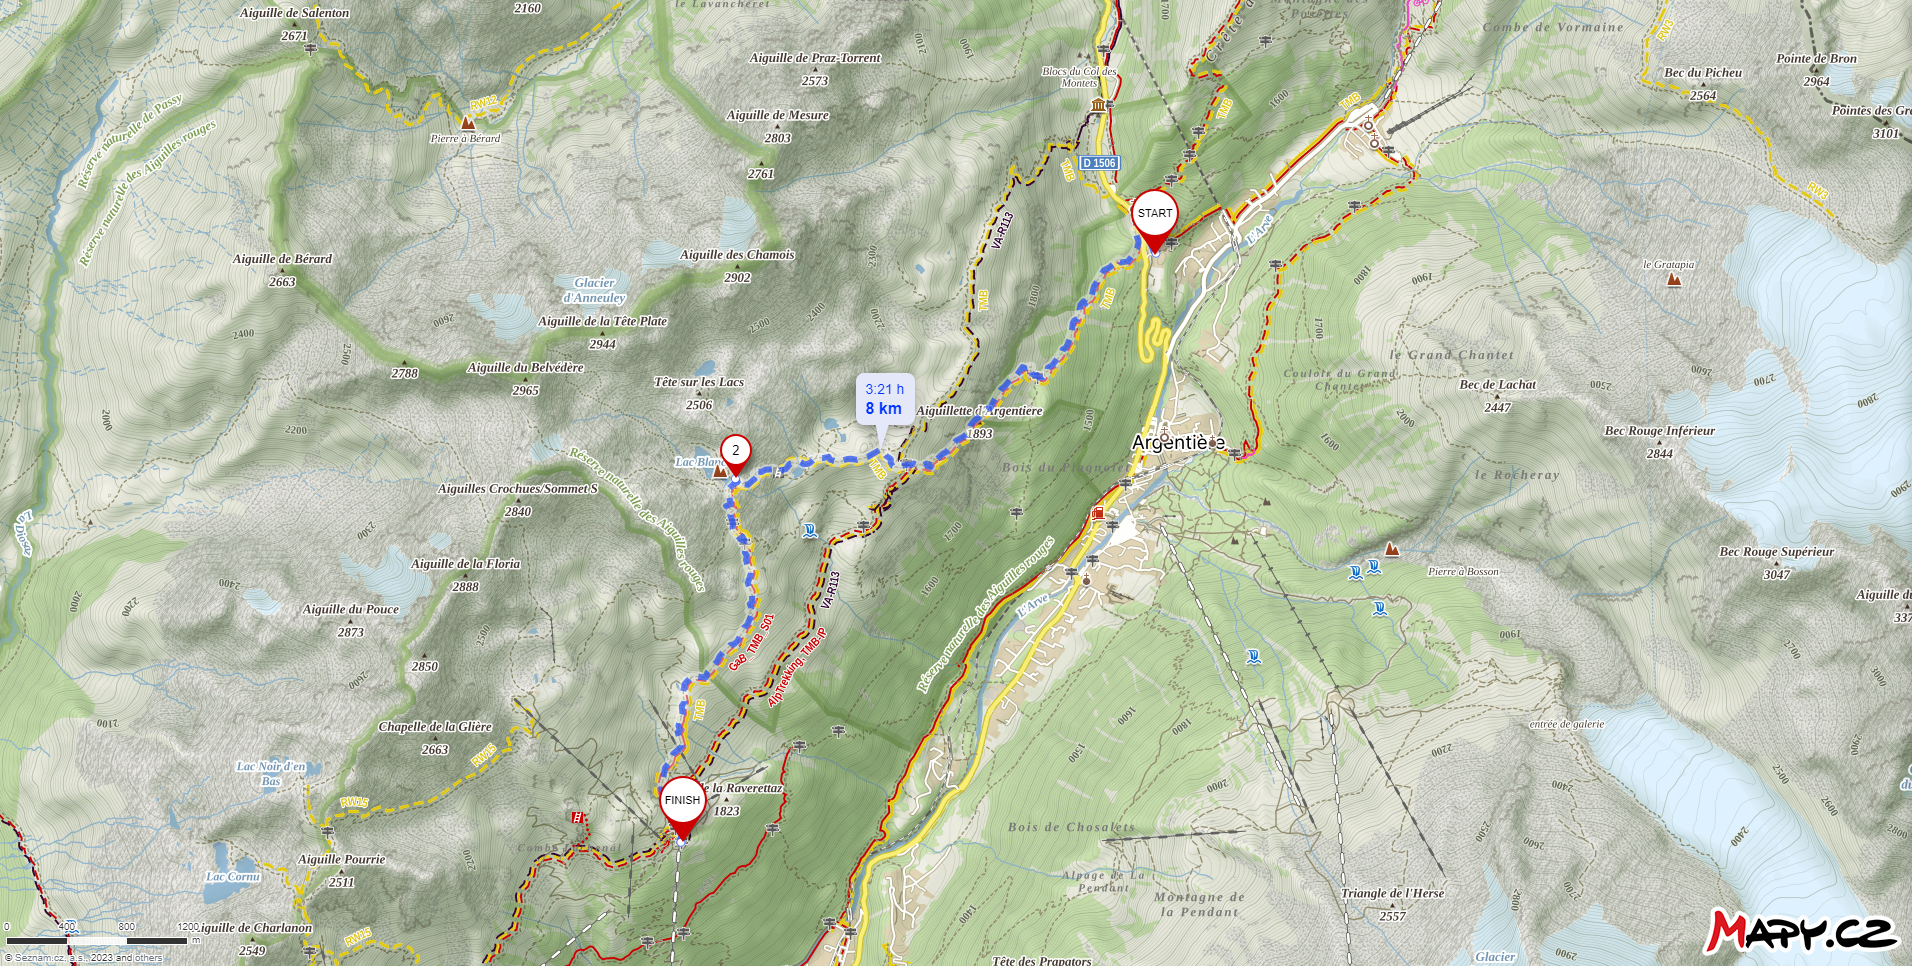
\includegraphics[width=10.0cm]{Figures/day_10.png}
	\caption[Trasa: den desátý]{Trasa 10. etapy (mapa převzata ze zdroje mapy.cz)}
	\label{Obr:day_10}
\end{figure} 
%% -------------------------------------------------- %%
\section{Etapa 11}
\subsubsection*{Celková délka}
\noindent Vzdálenost: 17,3\:km
\subsubsection*{Výchozí a koncový bod}
\noindent Výchozí bod: Flégère
\noindent Koncový bod: Les Houches
\subsubsection*{Převýšení}
\noindent Vystoupáno: 729\:m
\noindent Sestoupáno: 1\:605\:m
\subsubsection*{Časové plánování}
\noindent Předpokládaný čas túry: 7-9 hod.

Poslední etapa dlouhá 17,3\:km s vystoupáním 729\:m a sestoupáním 1605\:m.
\subsubsection*{Nouzová sestupová místa}
V poslední etapě jinou variantu cesty nemáme, ale budeme se pohybovat nad Chamonix, pokud tedy nastane problém nebude problém sjet dolu lanovkou.
\subsubsection*{Další informace}
Po 4,0\:km od startu narazíme na pramen vody, kde bude možné doplnit vodu a lehce si odpočinout. Po dalším 1,4\:km bude vyhlídkové místo. Dále po 2,0\:km bude možnost vyběhnout si na vrchol Le Brévent 2\:525\:m n. m. Zde je také konečná stanice lanovku s chatou, ve které si budeme moct sednout, popřípadě si dát jídlo. Nebo nás bude čekat chata za 2,7\:km. Po 2,0\:km od Le Brévent nas bude čekat další vrchol Tête de Bellachat s výškou 2\:276\:m. Od chaty Refuge de Bellachat nás poté bude od cíle dělit 6,8\:km. 
%% -------------------------------------------------- %%
%% -------------------- Picture --------------------- %%
%% -------------------------------------------------- %%
\begin{figure}[!hbt]
    \centering
    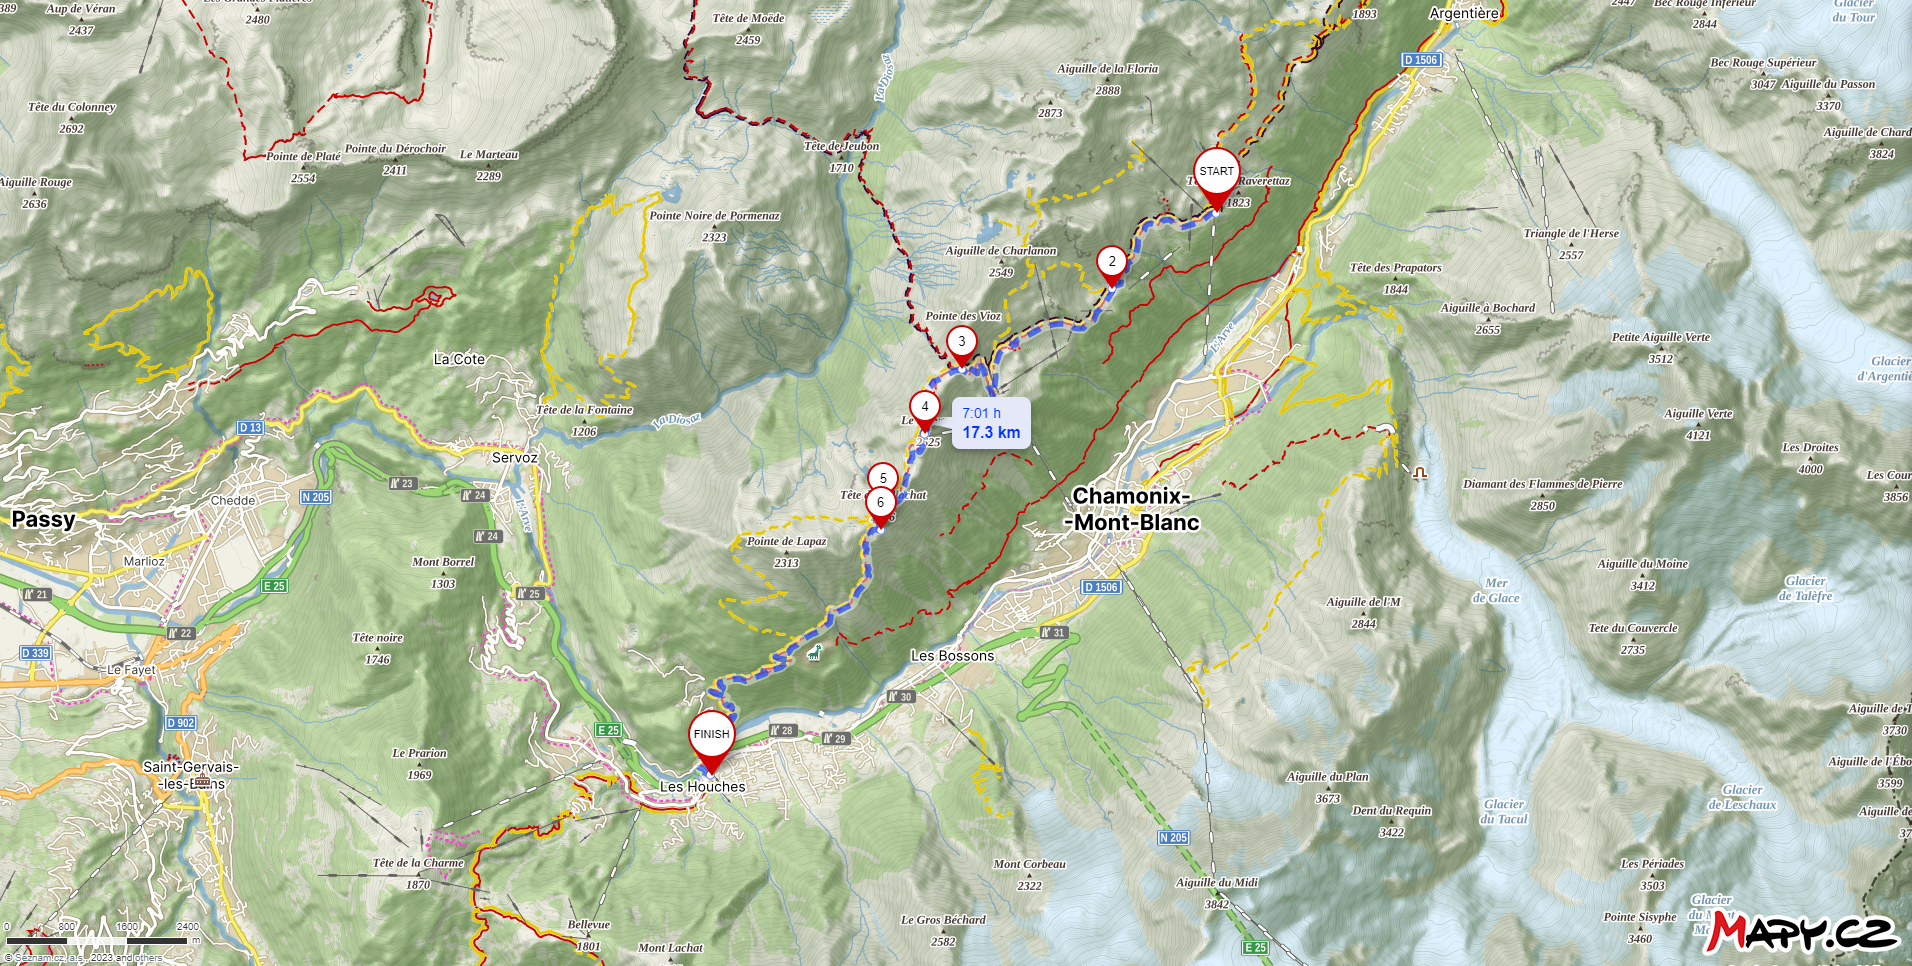
\includegraphics[width=10.0cm]{Figures/day_11.png}
    \caption[Trasa: den jedenáctý]{Trasa 11. etapy (mapa převzata ze zdroje mapy.cz)}
    \label{Obr:day_11}
\end{figure} 
%% -------------------------------------------------- %%
\section{Celková trasa}
\subsubsection*{Celková délka}
\noindent Vzdálenost: 166,1\:km
\subsubsection*{Převýšení}
\noindent Vystoupáno: 10\:650\:m
\noindent Sestoupáno: 10\:650\:m
\subsubsection*{Další informace}
Během přechodu bude začínat a končit na chatách, kde bude dostupná voda, také na trase potkáme mnoho pramenů, kde bude možnost vodu doplnit. Elektřina je dostupná na všech chatách. Mobilní signál může být v údolích horší, ale jinak se mimo signál vyskytovat nebudeme. Doplnit zásoby jídla bude možné hned několikrát, protože budeme procházet přes několik vesnic.
%% -------------------------------------------------- %%
%% -------------------- Picture --------------------- %%
%% -------------------------------------------------- %%
\begin{figure}[!hbt]
	\centering
	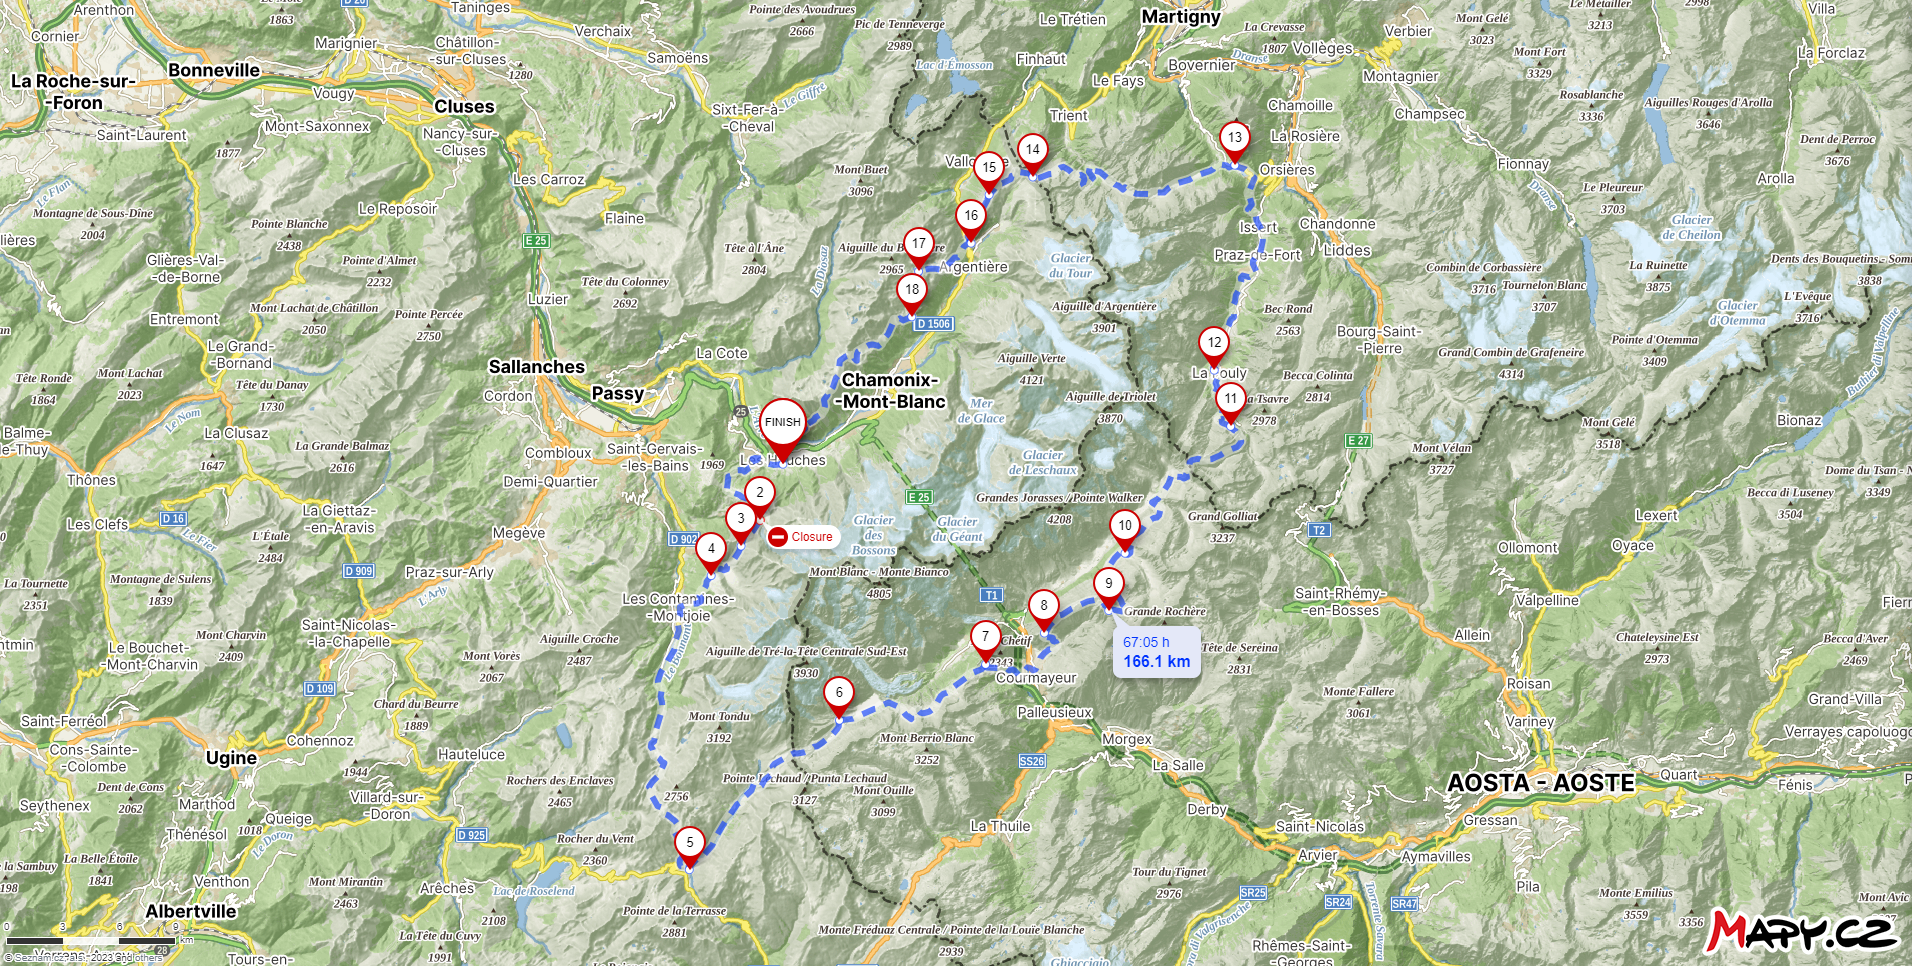
\includegraphics[width=10.0cm]{Figures/TMB.png}
	\caption[Trasa: Celková]{Celková trasa (mapa převzata ze zdroje mapy.cz)}
	\label{Obr:tmb}
\end{figure} 
%% -------------------------------------------------- %%